% TODO replace links each year
\newcommand{\PandaLink}{https://panda.uni-paderborn.de/course/view.php?id=54851}
\newcommand{\CalendarLink}{https://panda.uni-paderborn.de/calendar/view.php?view=month}
\newcommand{\Panda}{\href{\PandaLink}{Panda}}
\newcommand{\Youtube}{\href{https://www.youtube.com/watch?v=7sEHT-WX3ZE&list=PL4hJhdKDPIxha8So7muX2zfNUU8NBoiu3}{Youtube}}

\subsection{Who}

\begin{frame}{\myframetitle}
    % [image={\pic[width=5mm]{sp-icon}}]
	\myframeicon{\fancyqr{https://cs.uni-paderborn.de/se/teaching/software-product-lines}}
	\begin{fancycolumns}[animation=none]
		\begin{example}{Who Are You?}
			\begin{itemize}
				\item a \emph{Master student}
				\item looking for an \emph{elective subject} \deutsch{Wahlpflicht}
				\item enrolled in \emph{Computer Science}, \ldots
				\item interested in
				\begin{itemize}
					\item \emph{learning} about the basic principles of systematically managing software variability
					\item \emph{experimenting} with novel software engineering methods and tools
					\item getting in touch with current \emph{research} on software product lines
				\end{itemize}
			\end{itemize}
		\end{example}
	\nextcolumn
	\end{fancycolumns}
\end{frame}

\begin{frame}{\myframetitle}
	\begin{fancycolumns}[animation=none]
		\begin{note}{Who Are We?}
			\centering
			\href{https://www.uni-ulm.de/en/in/sp/team/thuem/}{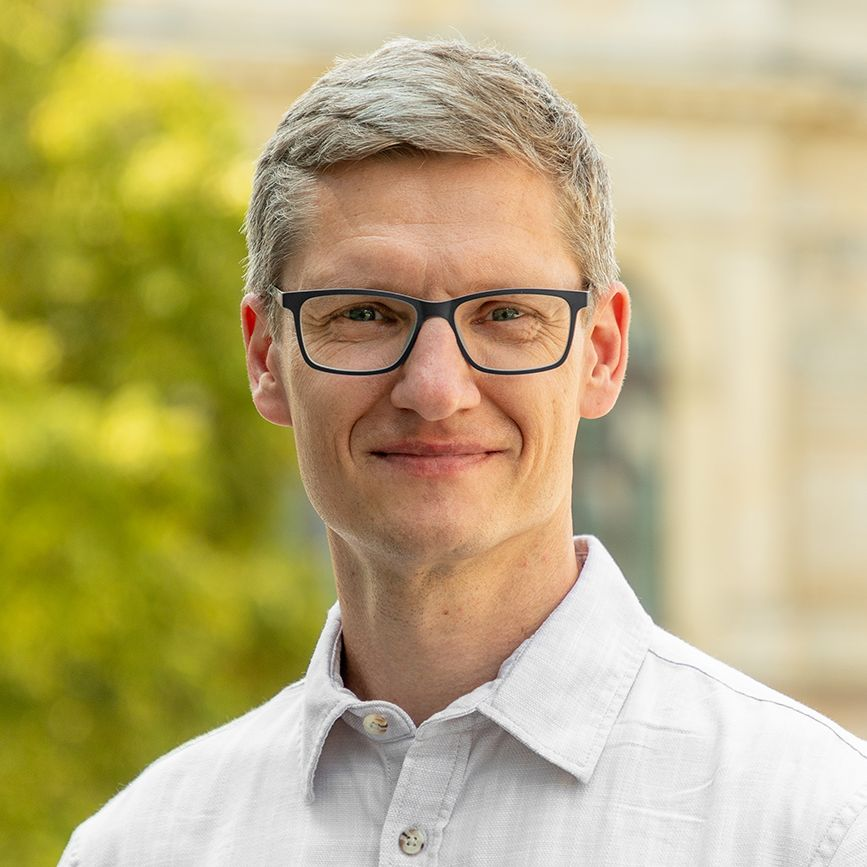
\includegraphics[height=40mm]{thomas-thuem}}\\[.5ex]
			\href{https://www.uni-ulm.de/en/in/sp/team/thuem/}{\emph{Thomas Thüm}}\\[.5ex]
			\small professor for software engineering\\[.5ex]
			FeatureIDE team leader
		\end{note}
	\nextcolumn
		\begin{note}{Who Are We?}
		    \centering
		    \href{https://www.uni-ulm.de/en/in/sp/team/paul-maximilian-bittner/}{
\includegraphics[height=40mm]{paul-bittner}}\\[.5ex]
			\href{https://www.uni-ulm.de/en/in/sp/team/paul-maximilian-bittner/}{\emph{Paul Bittner}}\\[.5ex]
			\small PhD student working on change analysis and formal languages for SPLs\\[.5ex]
		\end{note}
	\end{fancycolumns}
\end{frame}

\subsection{Where and When}

\begin{frame}{\myframetitle}
	\myframeicon{\fancyqr[image={\pic[width=10mm]{moodle-calendar}}]{\CalendarLink}}
	\begin{fancycolumns}
		\begin{definition}{Lecture}
			\begin{itemize}
				\item typically once per week
				\begin{itemize}
					\item exception: this week :)
					\item on \emph{Wednesday}, 09:15--10:45 (OK?)
					\item in room F2 211
					\item next lecture tomorrow
					\item see calendar on \Panda
				\end{itemize}
				\item usually held by Thomas
				\item \emph{slides} are available on \Panda
				\item \emph{videos} on \Youtube
				\item \emph{guest lecture} planned
			\end{itemize}
		\end{definition}
	\nextcolumn
		\begin{example}{Exercise}
			\begin{itemize}
				\item typically once per week
				\begin{itemize}
					\item on \emph{Tuesday}, 13:30--15:45 (OK?)
					\item in room F0 530
					\item starts on April 23rd
				\end{itemize}
				\item usually held by Paul
				\item exercise sheets are available on \Panda
				\begin{itemize}
					\item \emph{theoretical tasks}
					\item \emph{practical tasks}
				\end{itemize}
			\end{itemize}
		\end{example}
	\end{fancycolumns}
\end{frame}

%\subsection{Practical Tasks}

% master's theses, projects, seminars, dissertations, \ldots


\subsection{Taking the Exam, and Beyond}

\begin{frame}[label=Exam]{\myframetitle}
	\begin{fancycolumns}
		\begin{definition}{Exam}
			\begin{itemize}
				\item oral exam (or written exam if too many) %($\approx 20$ minutes)
				\item 2--3 exam days during lecture-free period
				\item FAQ at the end of each lecture
			\end{itemize}
		\end{definition}
		% \begin{definition}{Exam Eligibility \deutsch{Prüfungszulassung}} % TODO check
		\begin{definition}{Course Achievement \deutsch{Studienleistung}}
			\begin{itemize}
				\item pass all 6 practical tasks $\rightarrow$ eligible for exam
				\item develop your own software product line
				\item scope of topic is your choice
				\item submit own solution on GitLab
			\end{itemize}
		\end{definition}
		\begin{definition}{Grade Improvement \deutsch{Notenverbesserung}} % TODO check
			% $\geq 7$ points for active participation in exercise, lecture, and \Panda
			3 well-prepared presentations in the exercise
		\end{definition}
	\nextcolumn
		
%		\begin{note}{How to Withdraw from Your Exam?}
%			\begin{itemize}
%				\item 1+ weeks until exam: No reason required
%				\item Later: Provide proper reason
%			\end{itemize}
%		\end{note}	

		\begin{note}{How Does the Exercise Work?}
			\begin{itemize}
				\item Prepare all tasks you want to discuss at home
				\item \emph{You} prepare the exercise, we moderate!
			\end{itemize}
		\end{note}

		\begin{note}{Further Studies}
			\begin{itemize}
				\item \emph{projects}
				\item \emph{seminars}
				\item \emph{master's and PhD theses}
			\end{itemize}
			\ldots{} contact us!
		\end{note}
	\end{fancycolumns}
\end{frame}
